%%%%%%%%%%%%%%%%%%%%%%%%%%%%%%%%%%%%%%%%%%%%%%%%%%%%%%%%%%%%%%%%%%%%%%%%%%%%%%%%
%2345678901234567890123456789012345678901234567890123456789012345678901234567890
%        1         2         3         4         5         6         7         8

\documentclass[letterpaper, 10 pt, conference]{ieeeconf}  % Comment this line out if you need a4paper

\IEEEoverridecommandlockouts                              % This command is only needed if 
                                                          % you want to use the \thanks command

\overrideIEEEmargins                                      % Needed to meet printer requirements.

% See the \addtolength command later in the file to balance the column lengths
% on the last page of the document

% The following packages can be found on http:\\www.ctan.org
%\usepackage{graphics} % for pdf, bitmapped graphics files
%\usepackage{epsfig} % for postscript graphics files
%\usepackage{mathptmx} % assumes new font selection scheme installed
%\usepackage{times} % assumes new font selection scheme installed
%\usepackage{amsmath} % assumes amsmath package installed
%\usepackage{amssymb}  % assumes amsmath package installed
%\usepackage[numbers,sort&compress]{natbib}
%\usepackage{IEEEtran}
\usepackage{glossaries}

\title{\LARGE \bf
Impact of susceptibility distortions in connectivity analysis using dMRI
}


\author{Oscar Esteban$^{1,2}$, Alessandro Daducci$^{2}$, Emmanuel Caruyer$^{3}$, and Andr\'es Santos$^{1}$% <-this % stops a space
\thanks{$^{1}$Oscar Esteban is with PhD student of 
        {\tt\small oesteban@die.upm.es}}%
\thanks{$^{2}$        {\tt\small b.d.researcher@ieee.org}}%
}

% List of acronyms used in the text
\newacronym{mr}{MR}{magnetic resonance}
\newacronym{mri}{MRI}{magnetic resonance imaging}
\newacronym{dmri}{dMRI}{diffusion MRI}
\newacronym{fmri}{fMRI}{functional MRI}
\newacronym{dw}{DW}{diffusion weighted}
\newacronym{dti}{DTI}{diffusion tensor imaging}
\newacronym{t1}{T1}{T1-weighted}
\newacronym{t2}{T2}{T2-weighted}
\newacronym{csf}{CSF}{cerebrospinal fluid}
\newacronym{wm}{WM}{white matter}
\newacronym{gm}{GM}{grey matter}
\newacronym{epi}{EPI}{echo-planar imaging}
\newacronym{gre}{GRE}{gradient echo sequence}
\newacronym{fa}{FA}{fractional anisotropy}
\newacronym{md}{MD}{mean diffusivity}
\newacronym{adc}{ADC}{apparent diffusion coefficient}
\newacronym{acwe}{ACWE}{active contours without edges}
\newacronym{adf}{ADF}{active deformation field}
\newacronym{map}{MAP}{maximum a posteriori}
\newacronym{snr}{SNR}{signal-to-noise ratio}
\newacronym{pve}{PVE}{partial volume effect}
\newacronym{roi}{ROI}{region of interest}
\newacronym{mrf}{MRF}{Markov Random Field}
\newacronym{psf}{PSF}{point-spread function}
\newacronym{se}{SE}{Surface error}
\newacronym{wi}{WI}{Warping index}
\newacronym{nof}{NoF}{number of fibers}
\newacronym{hardi}{HARDI}{high angular resolution diffusion imaging}
\newacronym{tpm}{TPM}{tissue probability map}
\newacronym{fft}{FFT}{fast fourier transform}
\newacronym{vsm}{VSM}{voxel shift map}

\newacronym{fmb}{FMB}{fieldmap-based}
\newacronym{reb}{REB}{reversed encoding-based}
\newacronym{t2b}{T2B}{T2 registration-based}

\newacronym{frr}{FRR}{fiber recovery ratio}

\makeglossaries

%\acrodef{mr}[MR]{magnetic resonance}
%\acrodef{mri}[MRI]{magnetic resonance imaging}
%\acrodef{dwi}[DWI]{diffusion weighted imaging}
%\acrodef{dw}[DW]{diffusion weighted}
%\acrodef{dti}[DTI]{diffusion tensor imaging}
%\acrodef{t1}[T1]{T1-weighted}
%\acrodef{t2}[T2]{T2-weighted}
%\acrodef{csf}[CSF]{cerebrospinal fluid}
%\acrodef{wm}[WM]{white matter}
%\acrodef{gm}[GM]{grey matter}
%\acrodef{epi}[EPI]{echo-planar imaging}
%\acrodef{fa}[FA]{fractional anisotropy}
%\acrodef{md}[MD]{mean diffusivity}
%\acrodef{acwe}[ACWE]{active contours without edges}
%\acrodef{map}[MAP]{maximum a posteriori}
%\acrodef{snr}[SNR]{signal-to-noise ratio}
%\acrodef{pve}[PVE]{partial volume effect}
%\acrodef{roi}[ROI]{region of interest}



\begin{document}



\maketitle
\thispagestyle{empty}
\pagestyle{empty}


\begin{abstract}
Connectivity analysis on diffusion MRI data of the whole-brain
suffers from distortions caused by the standard 
echo-planar imaging acquisition strategies. %
%These artifacts are present at interfaces between tissues,
%due to the inhomogeneity of the field derived from the 
% discontinuity of magnetic susceptibility.
These images show characteristic geometrical deformations
and signal destruction that are an important pitfall
limiting the success of tractography algorithms.

Several retrospective correction techniques are readily
available. In this work, we use a digital phantom designed
for the evaluation of connectivity pipelines. We subject
the phantom to a ``theoretically correct'' and plausible
deformation that resembles the artifact under investigation.
We correct data back, with three standard methodologies
(namely fieldmap-based, reversed encoding-based, and
registration-based). Finally, we rank the methods based
on their geometrical accuracy, the dropout compensation,
and their impact on the resulting connectivity matrices.
\end{abstract}%
\begin{keywords}
susceptibility artifacts, diffusion MRI, tractography, connectivity.
\end{keywords}
\section{INTRODUCTION}

In-vivo whole-brain connectivity analysis has been a
research topic of high interest for the last
5 years. 
\Gls*{dmri} can be used to probe the
orientation of fiber bundles within the brain,
generally applying \gls*{epi} sequences.
After a signal reconstruction step, 
tractography algorithms draw a map of the sampled 
structures.
These maps can represent the actual trajectories
of fiber bundles (deterministic tractography) or
pixel-wise probability of connection to a certain origin
(probabilistic tractography). Finally, the
information about these connections is collected
into a network matrix that can be subjected to
the so-called ``connectome analysis''.

Among all the difficulties that such a complex workflow
raises \cite{jones_twenty-five_2010}, we will
address here the susceptibility-derived artifacts,
for which \Gls*{epi} schemes are specially sensitive.
As susceptibility changes at tissue interfaces,
so does the magnetic field. This inhomogeneities 
of the field translate in a highly distorted imaged 
anatomy and a significant signal  destruction of 
certain regions of the brain 
(e.g. the orbitofrontal lobe, for the proximity of the
air surrounding sinuses). This artifact has been
profoundly described, generally within the context of
functional MRI because it is usually acquired with 
\gls*{epi} as \gls*{dmri}. 

First approaches to
retrospective correction \cite{jezzard_correction_1995},
relied on an extra \gls*{mri} acquisition (so-called
\emph{field mapping}), that probes the inhomogeneity of the field.
A second theory-based breed of methodologies acquire a 
map of the \gls*{psf} of the \gls*{epi} readouts to correct 
for the artifact \cite{robson_measurement_1997}. 
Next generation of methodologies \cite{cordes_geometric_2000,
chiou_simple_2000}, make use of the acquisition of 
extra \gls*{epi} volumes 
with specific differences that enable correction, for instance
the opposed direction of the phase encoding gradients 
Finally, the last family of methodologies acquire an 
extra T2-weighted image, and use its anatomical correctness 
as reference to find the deformation map through nonlinear 
registration \cite{kybic_unwarping_2000,studholme_accurate_2000}.
Registration-based methods usually map
the T2 image to the so-called baseline (B0) volume 
of \gls*{dmri}. The choice of T2 is due to the strong
similarity of intensity distribution with the B0 of \gls*{dmri}
datasets. More recent works report extensions or combined
approaches of existing techniques
\cite{andersson_how_2003,zaitsev_point_2004,%
holland_efficient_2010,andersson_comprehensive_2012}.

Even though aforementioned techniques for distortion correction
have been studied \cite{zeng_image_2002,wu_comparison_2008},
the lack of a gold-standard limits the possible benchmarking 
strategies. Recently, \cite{irfanoglu_effects_2012} raised the question
of distortion-derived impacts in tractography.
In this work, we propose an evaluation framework
using a digital phantom designed for connectivity assessment.
This framework enabled us to compare several correction 
techniques and characterize their geometrical accuracy 
and the dropout compensation. Finally, we report their 
impact on subsequent tractography and resulting connectivity
matrices.
\section{METHODS}

\subsection{Digital Phantom}
Based on the fiber geometries of the digital phantom 
created for the \gls*{hardi} 
reconstruction Challenge held in ISBI 2013 
(San Francisco, US), we simulated high resolution 
(0.5mm isotropic) T1 (TE/TR=10/1500ms) and T2 
(TE/TR=90/5000ms) images, as well as two \gls*{dmri}
images (1.0mm isotropic, $b$=1200, 1 B0 image) with
32 and 64 evenly-distributed directions.
Diffusion is modeled by a restricted and a hindered
compartment, similar to \cite{assaf_composite_2005}.
The phantom includes \gls*{wm} fiber bundles,
\gls*{gm} and \gls*{csf}. Physical properties
(T1/T2 times in sec) used in simulation are
($0.832\pm0.010$ / $79\times10^{-3}\pm0.6\times10^{-3}$)
for \gls*{wm},
($1.331\pm0.013$ / $110\times10^{-3}\pm2.0\times10^{-3}$) for
\gls*{gm} and ($3.5\pm0.1$ / $0.25\pm0.01$) for \gls*{csf}.

\subsection{Theory-based synthetic distortion}
\label{sec:distortion}
\Gls*{fmb} methodologies use a map
of the field in the scanner. More precisely, the
phase difference between two subsequent samplings
of the fieldmap. With that information, it is possible
to compute the theoretical displacement that each
voxel undergoes, the so-called \gls*{vsm}. The
most prominent feature of this \gls*{vsm} is that all
the shifts have the same orientation (parallel to the
phase-encoding direction of the \gls*{epi}) and their
magnitude and direction depend on the \gls*{epi} 
gradient increments (or \emph{blips}), and the actual
phase difference at the voxel.

In order to create a realistic distortion, we
generated a synthetic phase-difference map 
consistent with the phantom, using the 
tools distributed with the \emph{FSL} package 
\cite{jenkinson_fsl_2012}  and
standard parameters ($\Delta$TE=2.46~ms. for the
field mapping and \emph{effective dwell time} of 
0.77~ms. for the \gls*{epi}).
We defined two regions of smooth dephasing and 
computed the corresponding \gls*{vsm}. Amplitude
of the dephasing maps can be modulated, enabling
us to evaluate the impact of the distortion magnitude.
We generated several \glspl*{vsm} with increasing
maximum shifts, ranging 3.80-7.60~mm, covering the
typical range of distortion observed in real datasets.

From these synthetic \glspl*{vsm}, we generated
the corresponding distorted \glspl*{dwi}, in two opposed
phase-gradient encoding directions. The second simulated
``acquisition'' of the same phantom was necessary 
for evaluating \gls*{reb} methods.

In summary, we generated 
a full gold-standard containing realistic T1 and T2
at high resolution, \glspl*{dwi} acquired in two
different phase encoding directions, and a ground-truth
\gls*{dwi} data, which is not available for real datasets
(\autoref{fig:phantom}).


\begin{figure}[thpb]
   \centering
   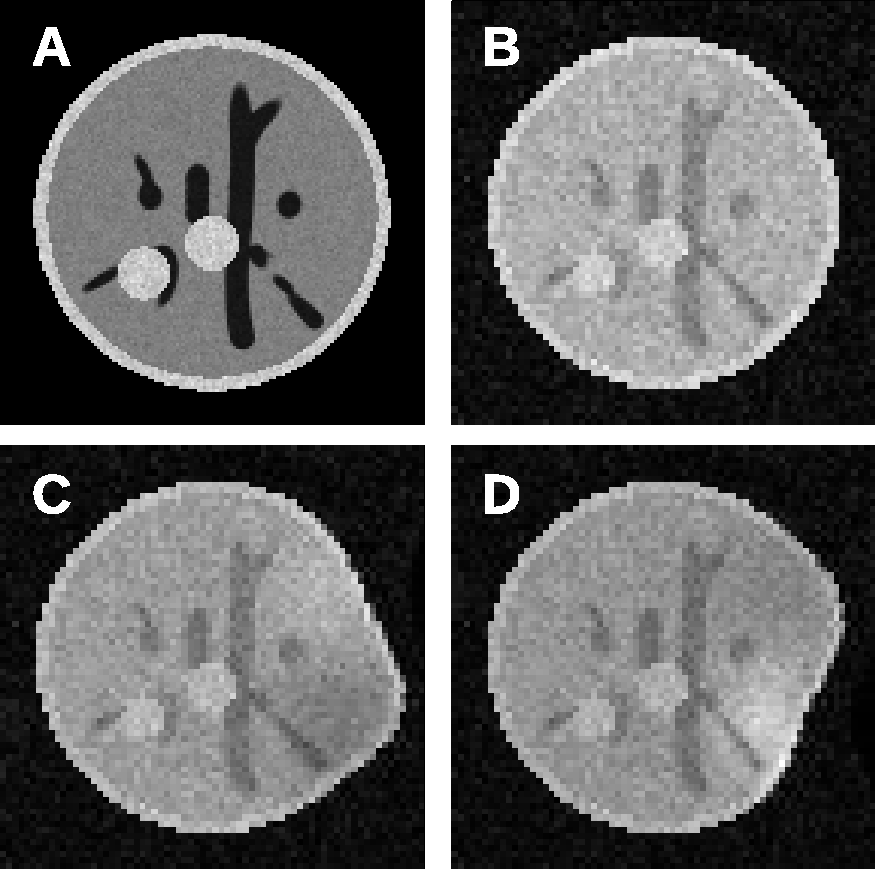
\includegraphics[width=0.95\columnwidth]{Fig01-Phantom}
   \caption{Ground-truth digital phantom.
   A) T2-weighted image; B) undistorted \textit{b0} volume;
   C, D) distorted \textit{b0} volumes with opposed phase 
   encoding directions, maximum displacement of 3.80~mm.}
   \label{fig:phantom}
\end{figure}

\subsection{Correction methods}
\label{sec:correction}
Three out of four methods presented in \autoref{sec:intro}
were tested on the evaluation framework. 

\Gls*{fmb} correction
is essentially the same as the one used for generating the 
distortion, on the inverse direction. Normally distributed 
noise was added to the fieldmap (for a signal-to-noise 
ratio of 20dB) before correction.

For \Gls*{reb} correction, we made use of the implementation found 
in \emph{FSL} (\texttt{topup})
that demands for the \textit{b0} of the reverse-encoding simulation.
In this second case, the \gls*{vsm} is inferred from the differences
between the two corresponding \textit{b0}.

Finally, for evaluating \Gls*{t2b},
we fine-tuned \emph{ANTs} \cite{avants_ants:_2013},
in order to register \textit{b0} to T2. To this end, we used a
multi-resolution scheme with 3 levels of subsampling and smoothing,
mutual information metric, and symmetric diffeomorphic transform 
(\texttt{SyN}). Several configurations of kernel widths for the 
regularization smoothers were tested, and finally selected 
0.5/1.0 voxels (gradient/deformation fields, respectively) 
for its best result. Additionally, undistorted images are 
corrected for dropout using the determinant
of the Jacobian of the deformation field.

\subsection{Evaluation}
\label{sec:evaluation}
The original phantom, one distorted version, and
the corrected instances are then connected to a
\gls*{dwi} reconstruction and tractography pipeline.
Additionally, the original tissue probability maps
are also distorted and corrected to provide tractography
with the required \gls*{wm} masks.
These maps are also used in a final assessment module.

The framework provides two different options for
\gls*{dwi} reconstruction and deterministic tractography.
Firstly, \emph{Diffusion Toolkit} \cite{wang_diffusion_2007}
for \gls*{dti}, is configured with 10 random
seeds per voxel by default. Secondly, \emph{MRTrix}
\cite{tournier_mrtrix:_2012} for \gls*{hardi}, with
default parameters set to use constrained spherical
deconvolution, maximum harmonic order of 6, and 150000
desired tracks.
For both options, the seeding regions can be set to use
either the distorted-corrected \gls*{wm} mask, or the 
regions used to generate the ground-truth. This second
seeding strategy mimics the usual procedure on real 
data, where regions are typically mapped from the
anatomically correct T1.

The evaluation framework is completed by automated 
assessment modules. We evaluated three characteristics
of the correction methods. 
Firstly, we assessed the geometrical correctness
reporting overlap indices of three tissue
probability maps (namely \gls*{csf}, \gls*{wm},
and \gls*{gm}), weighting the average by tissue
volumes.
Secondly, to evaluate the quality of the actual 
signal dropout correction, we studied the 
similarity volume by volume computing the $\ell_1$-norm
correlation index. We report this score
on the \textit{b0} and the average of the remaining \gls*{dwi}
volumes. Thirdly, we studied the impact on the
connectivity matrices reporting the number of
false positives (inexistent connections in the
gold-standard) and false negatives (or connections
lost).
\section{RESULTS}
\label{sec:results}

All the modules described in the previous section were
conveniently integrated in workflows using \emph{nipype}
\cite{gorgolewski_nipype:_2011}. The choice of this tool
grants the reproducibility of the experiments,
and the evaluation workflow is publicly released.
The results of the proposed experiments are summarized
in \autoref{fig:results} and \autoref{table:results}.
The remaining of this section provides extended descriptions
and interpretation of the results.

\begin{figure*}[tpb]
   \centering
   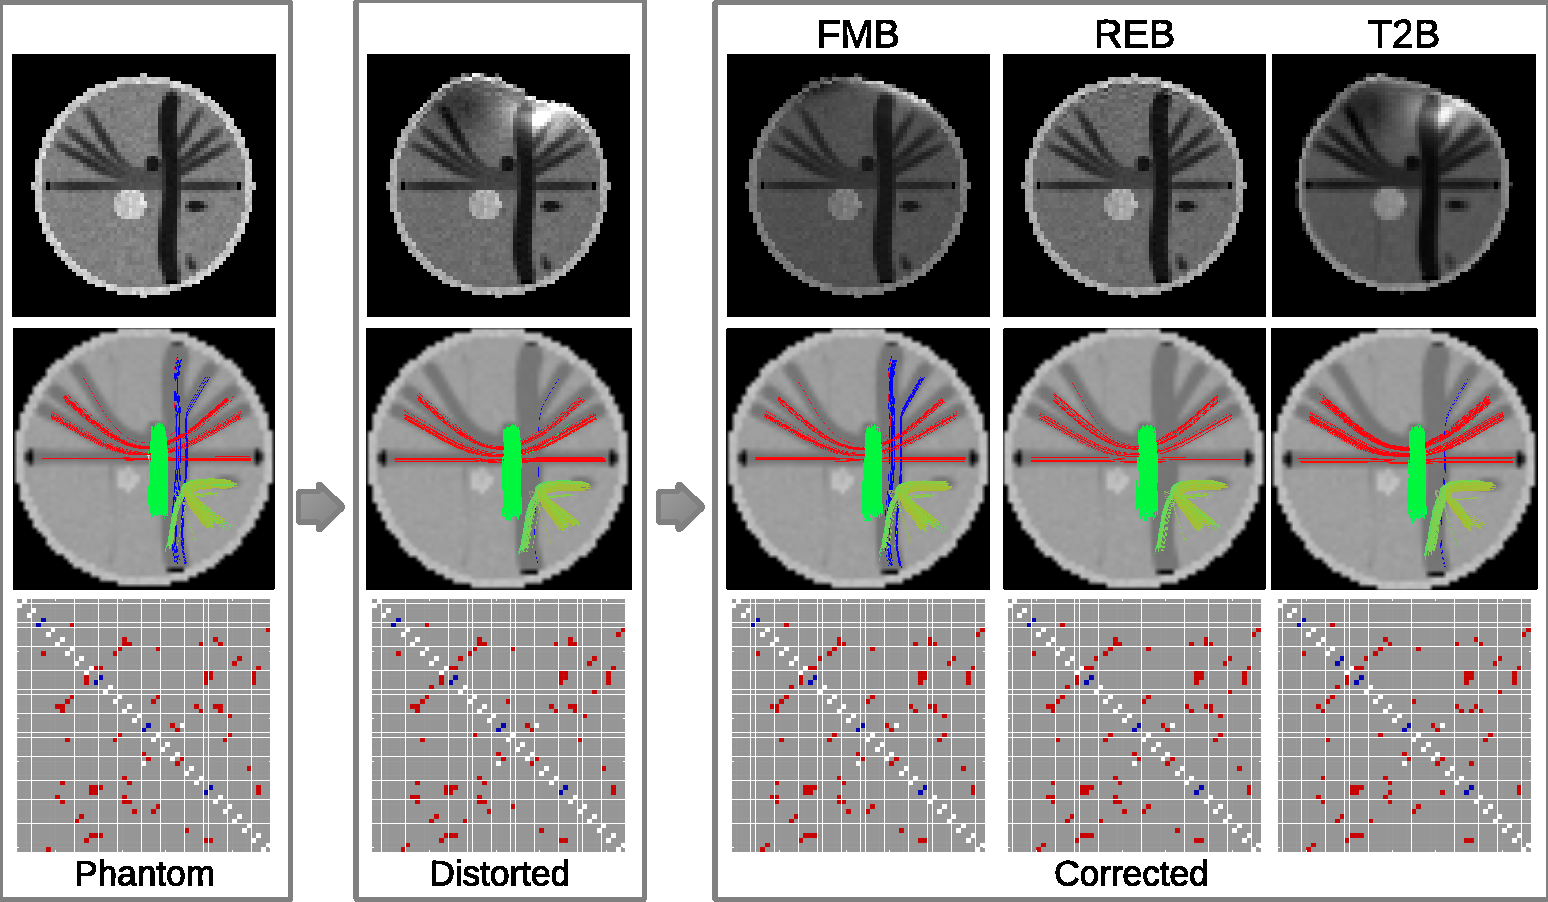
\includegraphics[width=0.9\textwidth]{Fig02-Results}
   \caption{Visual evaluation of the correction methods.
   First row represents a coronal section of the \textit{b0} volume. 
   In second row, the outcome of tractography after filtering tracks
   that did not connect two regions.
   Third row shows the associated connectivity matrices. All the matrices
   are compared to the ground-truth connections in the phantom. The existing
   connections that were correctly detected at each step are depicted in white
   color. False positives have been marked in red and false negatives in blue.
   Gray color represents the true negatives (non-existent connections correctly detected).}
   \label{fig:results}
\end{figure*}


\subsection{Geometrical correctness and signal recovery}

A summary of quantitative results, computed for the \gls*{dti} 
dataset with maximum shift of 3.80~mm,
is provided in \autoref{table:results}.
The best scores were obtained with the \gls*{reb} 
method, followed by \gls*{fmb}. 
The clear difference of accuracy between \gls*{reb} and \gls*{fmb}
with respect to \gls*{t2b} infers the latter may not be
an appropriate method for susceptibility correction. 
The described performance was constant for \gls*{fmb} 
and \gls*{reb} along the different magnitudes of 
distortion evaluated (maximum phase-encoding direction 
shifts in the range of 3.80-7.60~mm).


\begin{table}[h]
\caption{Numerical results}
\label{table:results}
\begin{center}
\begin{tabular}{c||cc|cccc}
\hline
Method & \multicolumn{2}{c|}{Similarity (\%)} & \multicolumn{4}{c}{\gls*{fji} (\%)} \\
\hline
 & B0 & \glspl*{dwi} & Av. & \gls*{csf} & \gls*{wm} & \gls*{gm} \\
\hline
\gls*{fmb} & $80.05$ & $96.26\pm.06$ & $93.00$ & $88.57$ & $96.74$ & $94.02$ \\
\hline
\gls*{reb} & $91.00$ & $97.65\pm.03$ & $96.64$ & $94.31$ & $98.26$ & $96.75$ \\
\hline
\gls*{t2b} & $64.58$ & $90.10\pm.13$ & $79.19$ & $66.31$ & $89.85$ & $82.14$ \\
\hline
\end{tabular}
\end{center}
\end{table}

A second workflow investigated the similarity of the recovered
signal with respect to the original (undistorted).
In this second study, \gls*{reb} performed
better than the other two methods, as reported
in \autoref{table:results}. \gls*{reb} scored a $91.0\%$
similarity index for the \textit{b0} volume and an average $97.65\%$
for the remaining \glspl*{dwi}. Again, the second
qualified was \gls*{fmb}, which achieved very close results
for the \glspl*{dwi} ($96.26\%$) but not as good for the \textit{b0}
volume. Visual inspection of the recovered data confirms the 
presented quantitative results (\autoref{fig:results}, first row).


\begin{table}[!t]
\caption{Tractography and connectivity results.}
\label{table:results-tractography}
\begin{center}
\begin{tabular}{l||cccc}
\hline
 & \# tracks & length (mm) & FP & FN \\
\hline
Original & 735 & $40.87\pm13.55$ & 40 & 4 \\
\hline
Distorted & 878 & $40.54\pm13.73$ & 42 & 4 \\
\hline
\gls*{fmb} & 743 & $40.04\pm13.60$ & 43 & 4 \\
\hline
\gls*{reb} & 830 & $39.87\pm13.93$ & 44 & 4 \\
\hline
\gls*{t2b} & 825 & $41.44\pm12.85$ & 40 & 5 \\
\hline
\end{tabular}
\end{center}
\end{table}

\subsection{Impact on tractography and connectivity}

Connectivity matrices derived from the \gls*{dti} dataset
were completely hindered by the high complexity of the 
fibers contained
in the phantom. Tractography discovered successfully only 4 out 
of 27 existing connections from the original (undistorted) data,
with more than 45 false connections.
With the \gls*{hardi} dataset (reconstructed with constrained 
spherical deconvolution) we found 23/27 connections,
but we still observed 40 false positives. Therefore, the 
experiments using the \gls*{dti} phantom were discarded. The
results presented in this subsection only refer to the 
\gls*{hardi} dataset.

Using the strongest distortion (maximum shift of 7.60~mm),
the number of detected connections
remained the same (23/27), slightly increasing the number of
false positives to 42. The immediate conclusion is that, with highly
complex anatomies (crossing, fanning, etc.) and limited number of
ground-truth connections, connectivity matrices are more sensitive 
to reconstruction and tractography than to distortions.

For the sake of completeness, \autoref{table:results-tractography}
reports the characteristic features of the tractography results
and connectivity matrices, for the fieldmap that caused a maximum
shift of 3.80~mm. Very similar results were obtained for
7.60~mm. This results, along with visual inspection
(\autoref{fig:results}, second and third rows), might point
to \gls*{fmb} as the best correction method.


\subsection{Discussion}

Even though all the surveyed methods produced visually 
sound results, our study suggested that \gls*{reb} is the 
most accurate method in terms of geometrical accuracy and
signal dropout recovery. 
The \gls*{t2b} method did not achieve the necessary high-standards
to recommend its use. Nonetheless, we understand that specific
methods with anisotropic regularization that completely
restrict deformations to the phase-encoding direction would perform
significantly better than the standard method presented.
Geometrical correctness of \gls*{dwi} data is fundamental 
in connectivity analysis to spatially locate the
regions which will define the nodes of the final connectivity
matrix.

Regarding tractography, this study revealed that signal
reconstruction and tractography algorithms masked the 
impact of susceptibility distortion on the final connectivity
matrices. Due to this effect, experiments performed on 
the \gls*{dti} phantom were discarded for comparison.
With the \gls*{hardi} dataset, the extracted 
connectivity matrix slightly
changed with distortion. Quantitative differences reported in
\autoref{table:results-tractography} could be more related
to the smoothing derived from interpolation implemented by
each method. Visual results might suggest that \gls*{fmb}
achieved better results.

Although we found connectivity matrices rather invariant with
respect distortion, they are suspected to be significantly
impacted by the susceptibility artifact on real data 
\cite{irfanoglu_effects_2012}.
This hypothesis points to the need of more appropriate 
phantoms with denser connectivity matrices.
State of the art phantoms for tractography usually present a
discrete set of simulated fiber bundles that translate in 
very sparse fiber-endings regions and connectivity matrix.
In the real case, the surface limiting the tracks is densely 
covered by the regions mapped from the anatomical 
dataset, what leads to larger sensitivity with respect 
deformations.

A possible limitation of this work is that \gls*{fmb} is
used for both synthesis and correction of the distortion.
However, practical reasons (i.e. noise, signal dropout)
impede perfect geometrical correction with \gls*{fmb}.
Moreover, \gls*{reb} performed more accurately 
than \gls*{fmb}.

Future extensions of this work will include a 
refined digital phantom. Additional lines for this
work will evaluate different realizations of the 
synthetic phase-difference map, to better characterize
the phenomenon. Also, the framework can be enhanced 
for studying the impact of other artifacts as 
subject's motion or eddy currents-derived distortions.
\section{CONCLUSION}

This paper proposes an evaluation framework to
comprehensively analyze the impact of susceptibility
induced distortion on tractography from \gls*{dmri}
data. Inaccuracy on tractography leads to significant
errors in posterior connectivity analyses of the
whole-brain, specially in distortion affected regions.
We publicly release the framework and also contribute
with the evaluation of three widely-used available
correction methodologies. We conclude that the 
\gls*{reb} method resulted the first method in the 
proposed rankings (geometric correctness, signal loss
recovery and tractography impact), with the drawback
of demanding some extra \gls*{dmri} data.


\addtolength{\textheight}{-12cm}   % This command serves to balance the column lengths
                                  % on the last page of the document manually. It shortens
                                  % the textheight of the last page by a suitable amount.
                                  % This command does not take effect until the next page
                                  % so it should come on the page before the last. Make
                                  % sure that you do not shorten the textheight too much.

%%%%%%%%%%%%%%%%%%%%%%%%%%%%%%%%%%%%%%%%%%%%%%%%%%%%%%%%%%%%%%%%%%%%%%%%%%%%%%%%



%%%%%%%%%%%%%%%%%%%%%%%%%%%%%%%%%%%%%%%%%%%%%%%%%%%%%%%%%%%%%%%%%%%%%%%%%%%%%%%%



%%%%%%%%%%%%%%%%%%%%%%%%%%%%%%%%%%%%%%%%%%%%%%%%%%%%%%%%%%%%%%%%%%%%%%%%%%%%%%%%
%\section*{APPENDIX}
%
%Appendixes should appear before the acknowledgment.
%
%\section*{ACKNOWLEDGMENT}
%
%The preferred spelling of the word �acknowledgment� in America is without an �e� after the �g�. Avoid the stilted expression, �One of us (R. B. G.) thanks . . .�  Instead, try �R. B. G. thanks�. Put sponsor acknowledgments in the unnumbered footnote on the first page.



%%%%%%%%%%%%%%%%%%%%%%%%%%%%%%%%%%%%%%%%%%%%%%%%%%%%%%%%%%%%%%%%%%%%%%%%%%%%%%%%

\bibliographystyle{IEEEtran}
% argument is your BibTeX string definitions and bibliography database(s)
\bibliography{IEEEabrv,99-references}



\end{document}
